\subsection{Experiment 3: Domain and Structural Transfer in Coin City}
\label{sec:exp3}

Experiment~3 extends Coin City from in-context inference to transfer after
training. Table~\ref{tab:exp3-training-policies} (Appendix~\ref{app:exp3-coin-structural})
defines the four training policies; Figure~\ref{fig:exp3-transfer-grid} shows the
four evaluation cells:
policies train only on Coin City/Structure~A, then face a domain shift, a
mechanism shift, and both together. Equations, parameters, mediator names, and
structure labels are withheld, while complete reference systems and a qualitative
description provide indirect pathway evidence
(Appendix~\ref{app:exp3-coin-structural}).

The registered endpoint is round 300 with greedy and five-draw stochastic
decoding over three models. The Qwen3-4B subset is complete under both
decoding regimes: all nine trained runs and the untrained endpoint share the same
1,440-task evaluation. The Qwen3-8B and Llama-3.1-8B confirmatory grids were
incomplete at the analysis freeze, so the cross-model endpoint is unavailable.

% Experiment 3 transfer results, laid out on the same 2x2 grid as the design
% figure (Figure~\ref{fig:exp3-transfer-grid}) so the reader reads results in the
% cells they were introduced in: mechanism down the rows, surface domain across
% the columns, the trained cell shaded blue and the three held-out cells green.
%
% Every number comes from tables/exp3_coin_qwen3_4b_stochastic_data.tex,
% regenerated by coin_city_structural/make_qwen3_4b_endpoint_outputs.py. Bar
% lengths share one scale
% (\cciPeak) across all four cells so cells are comparable by eye. Do not put
% formatting logic here: emphasis on an interval that excludes zero is decided
% by the generator and arrives pre-set in \cci*delta.
% generated by coin_city_structural/make_qwen3_4b_endpoint_outputs.py -- do not edit
\newcommand{\cciPeak}{8.53}
\newcommand{\cciIDbase}{3.82}
\newcommand{\cciIDless}{2.56}
\newcommand{\cciIDprior}{0.79}
\newcommand{\cciIDcausal}{0.58}
\newcommand{\cciIDdelta}{\textbf{0.21} [0.11, 0.32]}
\newcommand{\cciIDsig}{1}
\newcommand{\cciDomainbase}{8.53}
\newcommand{\cciDomainless}{5.23}
\newcommand{\cciDomainprior}{1.91}
\newcommand{\cciDomaincausal}{1.68}
\newcommand{\cciDomaindelta}{\textbf{0.23} [0.04, 0.38]}
\newcommand{\cciDomainsig}{1}
\newcommand{\cciStructurebase}{2.66}
\newcommand{\cciStructureless}{3.59}
\newcommand{\cciStructureprior}{2.53}
\newcommand{\cciStructurecausal}{2.34}
\newcommand{\cciStructuredelta}{\textbf{0.19} [0.02, 0.35]}
\newcommand{\cciStructuresig}{1}
\newcommand{\cciJointbase}{6.15}
\newcommand{\cciJointless}{6.76}
\newcommand{\cciJointprior}{4.81}
\newcommand{\cciJointcausal}{4.49}
\newcommand{\cciJointdelta}{\textbf{0.32} [0.13, 0.49]}
\newcommand{\cciJointsig}{1}

\begin{figure}[t]
\centering
\definecolor{gCityFill}{HTML}{E8F2FB}
\definecolor{gCityEdge}{HTML}{4F7EA8}
\definecolor{gHarborEdge}{HTML}{3F8E82}
\definecolor{gTestFill}{HTML}{E7F4EA}
\definecolor{gTestEdge}{HTML}{6FA97F}
\definecolor{gTestChip}{HTML}{5E9470}
\definecolor{gCoinFill}{HTML}{FFF2CC}
\definecolor{gCoinRim}{HTML}{D6B656}
\definecolor{gInk}{HTML}{3F4550}
\definecolor{gMute}{HTML}{8A93A3}
\definecolor{gBarBase}{HTML}{C3CBD4}
\definecolor{gBarLess}{HTML}{A9B4C0}
\definecolor{gBarPrior}{HTML}{7C93AD}
\definecolor{gBarCausal}{HTML}{4F7EA8}
\newcommand{\gcoincity}[2]{%
  \begin{scope}[shift={(#1,#2)},scale=0.70]
    \fill[gCoinFill] (0,0) circle (.37);
    \draw[gCoinRim,line width=.75pt] (0,0) circle (.37);
    \fill[gCityEdge] (-.23,-.18) rectangle (-.10,.04);
    \fill[gCityEdge] (-.07,-.18) rectangle (.07,.16);
    \fill[gCityEdge] (.10,-.18) rectangle (.24,.09);
    \draw[gCityEdge,line width=.65pt] (-.27,-.19)--(.27,-.19);
  \end{scope}}
\newcommand{\gcoinharbor}[2]{%
  \begin{scope}[shift={(#1,#2)},scale=0.70]
    \fill[gCoinFill] (0,0) circle (.37);
    \draw[gCoinRim,line width=.75pt] (0,0) circle (.37);
    \fill[gHarborEdge] (-.24,-.05)--(.24,-.05)--(.15,-.18)--(-.15,-.18)--cycle;
    \draw[gHarborEdge,line width=.7pt] (-.01,-.05)--(-.01,.15)--(.15,.02)--(-.01,.02);
    \draw[gHarborEdge,line width=.55pt]
      (-.26,-.24)..controls(-.18,-.19)and(-.10,-.29)..(-.02,-.24)
      ..controls(.06,-.19)and(.14,-.29)..(.26,-.24);
  \end{scope}}
% One results card. #1 cx, #2 cy, #3 cell name, #4 chip text, #5 chip fill,
% #6..#9 base/structureless/prior/causal MAE, #10 preformatted contrast.
\newcommand{\gcard}[9]{%
  \node[cellname] at (#1-2.66,#2+0.78) {#3};
  \node[chip, fill=#5] at (#1+2.66,#2+0.78) {#4};
  \foreach \arm/\val/\col/\dy in {%
      base/#6/gBarBase/0.40, structureless/#7/gBarLess/0.12,
      prior/#8/gBarPrior/-0.16, causal/#9/gBarCausal/-0.44}{%
    \node[armlab] at (#1-2.66,#2+\dy) {\arm};
    \fill[\col, rounded corners=1pt]
      (#1-0.95,#2+\dy-0.075) rectangle (#1-0.95+\val*2.95/\cciPeak,#2+\dy+0.075);
    \node[armval] at (#1-0.83+\val*2.95/\cciPeak,#2+\dy) {\val};}}
\resizebox{\linewidth}{!}{%
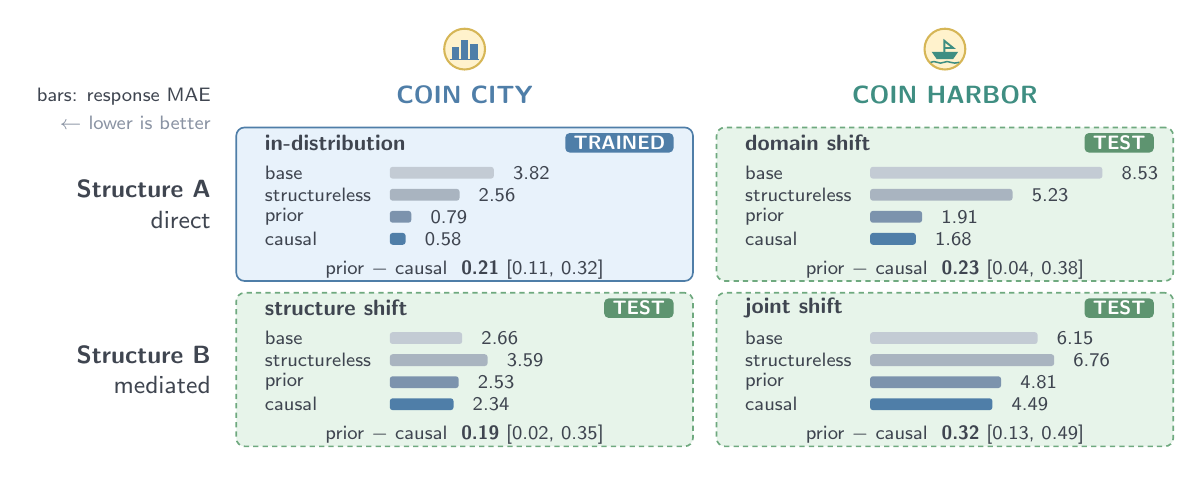
\begin{tikzpicture}[
  x=1cm, y=1cm,
  card/.style={rounded corners=3pt, minimum width=5.80cm, minimum height=1.95cm,
    line width=.6pt, inner sep=0pt},
  traincard/.style={card, draw=gCityEdge, fill=gCityFill},
  testcard/.style={card, draw=gTestEdge, fill=gTestFill,
    dash pattern=on 1.9pt off 1.5pt},
  dname/.style={anchor=south, font=\sffamily\bfseries\small},
  rname/.style={anchor=east, align=right, font=\sffamily\small, text=gInk},
  cellname/.style={anchor=west, font=\sffamily\bfseries\footnotesize, text=gInk},
  chip/.style={anchor=east, rounded corners=1.6pt, draw=none, text=white,
    inner xsep=3pt, inner ysep=1.1pt, font=\sffamily\bfseries\scriptsize},
  armlab/.style={anchor=west, font=\sffamily\scriptsize, text=gInk},
  armval/.style={anchor=west, font=\sffamily\scriptsize, text=gInk},
  delta/.style={anchor=center, font=\sffamily\scriptsize, text=gInk},
  legend/.style={anchor=east, font=\sffamily\scriptsize},
]
% ---- domain columns ------------------------------------------------------
\gcoincity{2.90}{3.22}
\gcoinharbor{9.00}{3.22}
\node[dname, text=gCityEdge]   at (2.90,2.40) {COIN CITY};
\node[dname, text=gHarborEdge] at (9.00,2.40) {COIN HARBOR};

% ---- what the bars mean, and which way is good --------------------------
\node[legend, text=gInk]  at (-0.20,2.62) {bars: response MAE};
\node[legend, text=gMute] at (-0.20,2.28) {$\leftarrow$ lower is better};

% ---- mechanism rows ------------------------------------------------------
\node[rname] at (-0.20,1.25) {\textbf{Structure A}\\ direct};
\node[rname] at (-0.20,-0.85) {\textbf{Structure B}\\ mediated};

% ---- the four result cards ----------------------------------------------
\node[traincard] at (2.90,1.25) {};
\node[testcard]  at (9.00,1.25) {};
\node[testcard]  at (2.90,-0.85) {};
\node[testcard]  at (9.00,-0.85) {};

\gcard{2.90}{1.25}{in-distribution}{TRAINED}{gCityEdge}
  {\cciIDbase}{\cciIDless}{\cciIDprior}{\cciIDcausal}
\node[delta] at (2.90,0.42) {prior $-$ causal\ \ \cciIDdelta};

\gcard{9.00}{1.25}{domain shift}{TEST}{gTestChip}
  {\cciDomainbase}{\cciDomainless}{\cciDomainprior}{\cciDomaincausal}
\node[delta] at (9.00,0.42) {prior $-$ causal\ \ \cciDomaindelta};

\gcard{2.90}{-0.85}{structure shift}{TEST}{gTestChip}
  {\cciStructurebase}{\cciStructureless}{\cciStructureprior}{\cciStructurecausal}
\node[delta] at (2.90,-1.68) {prior $-$ causal\ \ \cciStructuredelta};

\gcard{9.00}{-0.85}{joint shift}{TEST}{gTestChip}
  {\cciJointbase}{\cciJointless}{\cciJointprior}{\cciJointcausal}
\node[delta] at (9.00,-1.68) {prior $-$ causal\ \ \cciJointdelta};
\end{tikzpicture}%
}
\caption{\textbf{Qwen3-4B Coin City transfer at round 300 under five-draw
stochastic decoding}, on the design grid of
Figure~\ref{fig:exp3-transfer-grid}. Each bar is response MAE after averaging
five draws within task and four evidence depths; shorter is better, and trained
arms average three seeds. The paired seed-first prior-minus-causal difference is
printed under each cell, in bold where its 95\% interval excludes zero; positive
values favor episode-specific reward.}
\label{fig:exp3-transfer-results}
\end{figure}


\textbf{Episode-specific reward improves the hardest transfer forecast.}
Under five-draw stochastic decoding, joint new-domain/new-structure MAE is $6.15$
for the untrained base, $6.76$ for structureless training, $4.81$ for
population-prior training, and $4.49$ for causal training. The paired
prior-minus-causal difference is $.319$ $[.134,.489]$
(Figure~\ref{fig:exp3-transfer-results}). Causal training has the lowest point
estimate in all four cells, and all four intervals exclude zero. Draws are
averaged within task before the seed-first bootstrap. Every trained forecast
parses; the base parse rate is 99.97\%.

Greedy decoding agrees directionally. Its joint-cell MAEs are $6.09$, $6.69$,
$4.77$, and $4.59$, respectively, with a prior-minus-causal difference of $.174$
$[.039,.316]$. Causal training again has the lowest point estimate in all four
cells; the interval excludes zero for the in-distribution and joint-transfer
cells, but not for the domain-only or structure-only cells. The complete greedy
grid appears in Appendix~\ref{app:exp3-coin-qwen4b}.

\textbf{The error gain does not establish recovery of the unseen dynamics.}
In the joint cell, correct, absent, and misleading hints yield stochastic
causal MAE of $4.49$, $4.64$, and $4.81$, so qualitative-hint separation remains
small. The greedy values are $4.59$, $4.68$, and $4.86$. A nearest-pathway
response-shape diagnostic identifies Structure~B for none of the stochastic
causal draws and only $.025$ of greedy causal forecasts, compared with $.873$ and
$.817$ for the corresponding, less accurate base forecasts. Thus,
episode-aligned reward improves intervention forecasts, including under joint
transfer, but the result remains compatible with conservative response shrinkage
rather than reconstruction of the persistent mediator.

A separate completed Qwen3-4B study evaluates four held-out blocks spanning unseen
topologies, nonlinearities, mixed mechanism compositions, and parameter
extrapolation (Appendix~\ref{app:exp3-expanded-structural-ood}). Causal training
performs better under repeated sampling but not greedy decoding, and mechanism
classification remains near chance. We report this broader structural-transfer
test in the appendix and center Coin City because it directly extends
Experiment~2.

\subsection{Experiment 4: Transfer to Held-Out Historical Markets}
\label{sec:exp4}

Experiment~4 tests transfer on resolved events. Training, development, and sealed
test sets share no event families or normalized question templates. The test
contains 1,024 markets, and all 4,096 base and trained forecasts parse.

\begin{center}
\begin{minipage}{\linewidth}
\centering
\captionof{table}{\textbf{Historical-market training improves sealed-test
accuracy.} The test contains 1,024 markets. Lower is better; negative differences
favor the trained model.}
\label{tab:exp4-endpoint-results}
\scriptsize
\setlength{\tabcolsep}{3.5pt}
\resizebox{\linewidth}{!}{% Completed checkpoint-300 locked-test results, 2026-08-13.
% Source: reports/exp3b_locked_test_j30505540.summary.json.
\begin{tabular}{lrrrrr}
\toprule
Forecaster & Updates & Brier $\downarrow$ & $\Delta$ base & $\Delta$ market & Log loss $\downarrow$ \\
\midrule
Untrained Qwen3-4B       & 0   & .1316 & ---    & +.0179 & .5114 \\
Trained mean             & 300 & .1159 & -.0157 & +.0022 & .3960 \\
\midrule
Contemporaneous market   & --- & .1137 & -.0179 & ---    & .3658 \\
Market + train-fit logit & --- & .1123 & -.0193 & -.0014 & .3605 \\
\bottomrule
\end{tabular}
}
\end{minipage}
\end{center}

\textbf{Every training seed improves on the untrained model.}
Mean Brier score falls from $.1316$ to $.1159$, a difference of $-.0157$
$[-.0253,-.0067]$; log loss falls from $.5114$ to $.3960$. Exact event or
question-template repetition across splits cannot explain the gain.

\textbf{The trained model approaches, but does not surpass, the market.}
Training closes 88\% of the base-to-market Brier gap. Its difference from the
contemporaneous market is $.0022$ $[-.0026,.0072]$ and from train-only logistic
recalibration is $.0036$ $[-.0013,.0087]$. Both intervals include zero.

\textbf{Training changes directional consistency more than selectivity.}
On fixed initial forecasts, training raises directional consistency by $.0101$
$[.0004,.0207]$. The sensitivity difference, with interval $[-.07,.48]$, is
unresolved. The historical study shows accuracy transfer relative to the untrained
checkpoint. It does not show performance beyond market prices or a general change
in evidence selectivity.
